
\documentclass[a4paper,12pt]{article}

% === PODSTAWOWE USTAWIENIA ===
\usepackage[utf8]{inputenc}
\usepackage[T1]{fontenc}
\usepackage[polish]{babel}
\usepackage{geometry}
\usepackage{tabularx}
\usepackage{booktabs}
\geometry{top=2.5cm, bottom=2.5cm, left=2.5cm, right=2.5cm}
\usepackage{cite}

% === KOLORY ===
\usepackage[dvipsnames,table]{xcolor}

% Definicje kolorów dla poszczególnych rozdziałów
\definecolor{chap1}{RGB}{25,118,210}      % Niebieski - Wprowadzenie
\definecolor{chap1sub}{RGB}{33,150,243}   % Jasny niebieski
\definecolor{chap2}{RGB}{56,142,60}       % Zielony - Architektura
\definecolor{chap2sub}{RGB}{76,175,80}    % Jasny zielony
\definecolor{chap3}{RGB}{245,124,0}       % Pomarańczowy - Implementacja
\definecolor{chap3sub}{RGB}{255,152,0}    % Jasny pomarańczowy
\definecolor{chap4}{RGB}{123,31,162}      % Fioletowy - Frontend
\definecolor{chap4sub}{RGB}{156,39,176}   % Jasny fioletowy
\definecolor{chap5}{RGB}{198,40,40}       % Czerwony - Wdrożenie
\definecolor{chap5sub}{RGB}{229,57,53}    % Jasny czerwony
\definecolor{chap6}{RGB}{0,121,107}       % Morski - Wnioski
\definecolor{chap6sub}{RGB}{0,150,136}    % Jasny morski


% Kolory dla strony tytułowej
\definecolor{titleblue}{RGB}{13,71,161}
\definecolor{titlelightblue}{RGB}{25,118,210}
\definecolor{accentorange}{RGB}{255,111,0}

% Kolor dla kodu
\definecolor{codegray}{RGB}{245,245,245}
\definecolor{codeframe}{RGB}{200,200,200}

% === CZCIONKI I MIKROTYPOGRAFIA ===
\usepackage{lmodern}
\usepackage{microtype}
\usepackage{inconsolata}

% === PAKIETY DO GRAFIKI I WYKRESÓW ===
\usepackage{graphicx}
\usepackage{tikz}
\usetikzlibrary{shapes,arrows,positioning,calc,patterns,decorations.pathreplacing,shadows,backgrounds}
\usepackage{pgfplots}
\pgfplotsset{compat=1.18}

% === NAGŁÓWKI I STOPKI ===
\usepackage{fancyhdr}
\pagestyle{fancy}
\fancyhf{}
\fancyhead[L]{\nouppercase{\leftmark}}
\fancyhead[R]{\thepage}
\fancyfoot[C]{\footnotesize Uniwersytet Rzeszowski \textbullet\ Projekt Inżynierski \textbullet\ 2025/2026}
\renewcommand{\headrulewidth}{0.4pt}
\renewcommand{\footrulewidth}{0.4pt}
\setlength{\headheight}{18pt}

% === SEKCJE – KOLOROWE I CZYTELNE ===
\usepackage{titlesec}

% Licznik do śledzenia aktualnego rozdziału
\newcommand{\sectioncolor}{black}

% Format dla section (rozdział główny)
\titleformat{\section}
{\sffamily\LARGE\bfseries\color{\sectioncolor}}
{\colorbox{\sectioncolor}{\color{white}\parbox{1.5em}{\centering\thesection}}}{1em}{}
[\titlerule]

\titlespacing*{\section}{0pt}{3.5ex plus 1ex minus .2ex}{2.3ex plus .2ex}

% Format dla subsection
\titleformat{\subsection}
{\sffamily\Large\bfseries\color{\sectioncolor}}
{\thesubsection.}{1em}{}

\titlespacing*{\subsection}{0pt}{3.25ex plus 1ex minus .2ex}{1.5ex plus .2ex}

% Format dla subsubsection
\titleformat{\subsubsection}
{\sffamily\large\bfseries\color{\sectioncolor}}
{\thesubsubsection.}{1em}{}

\titlespacing*{\subsubsection}{0pt}{3.25ex plus 1ex minus .2ex}{1.5ex plus .2ex}

% === LISTINGI KODU – ESTETYCZNE I KOLOROWE ===
\usepackage{listings}

% Definicja języka JavaScript/TypeScript
\lstdefinelanguage{JavaScript}{
  keywords={typeof, new, true, false, catch, function, return, null, catch, switch, var, if, in, while, do, else, case, break, const, let, async, await, export, import, from, default, class, extends, constructor, this, super},
  keywordstyle=\color{blue!70!black}\bfseries,
  ndkeywords={class, export, boolean, throw, implements, import, this, interface, Promise, any, string, number},
  ndkeywordstyle=\color{purple!70!black}\bfseries,
  identifierstyle=\color{black},
  sensitive=false,
  comment=[l]{//},
  morecomment=[s]{/*}{*/},
  commentstyle=\color{gray}\ttfamily\itshape,
  stringstyle=\color{red!70!black}\ttfamily,
  morestring=[b]',
  morestring=[b]"
}

\lstdefinestyle{mystyle}{
    backgroundcolor=\color{codegray},
    basicstyle=\ttfamily\small,
    keywordstyle=\bfseries\color{blue!70!black},
    commentstyle=\itshape\color{gray},
    stringstyle=\color{red!70!black},
    numberstyle=\tiny\color{gray},
    numbers=left,
    numbersep=10pt,
    frame=single,
    rulecolor=\color{codeframe},
    breaklines=true,
    captionpos=b,
    abovecaptionskip=12pt,
    belowcaptionskip=10pt,
    xleftmargin=15pt,
    xrightmargin=10pt,
    columns=fullflexible,
    keepspaces=true,
    showstringspaces=false,
    tabsize=2
}
\lstset{style=mystyle}

% Obsługa polskich znaków w listingach
\lstset{
    literate={ą}{{\k{a}}}1 {ć}{{'c}}1 {ę}{{\k{e}}}1 {ł}{{\l{}}}1 {ń}{{'n}}1
             {ó}{{'o}}1 {ś}{{'s}}1 {ź}{{'z}}1 {ż}{{\.z}}1
             {Ą}{{\k{A}}}1 {Ć}{{'C}}1 {Ę}{{\k{E}}}1 {Ł}{{\L{}}}1 {Ń}{{'N}}1
             {Ó}{{'O}}1 {Ś}{{'S}}1 {Ź}{{'Z}}1 {Ż}{{\.Z}}1
}

% === POZOSTAŁE PAKIETY ===
\usepackage{float}
\usepackage{caption}
\usepackage{subcaption}
\usepackage{booktabs}
\usepackage{array}
\usepackage{multirow}
\usepackage{longtable}
\usepackage{pdflscape}
\usepackage{enumitem}
\usepackage{amsmath,amssymb}
\usepackage{algorithm}
\usepackage{algpseudocode}
\usepackage{tocloft}
\usepackage{setspace}
\onehalfspacing

% === USTAWIENIA HIPERŁĄCZY I METADANYCH PDF ===
\usepackage{hyperref}
\hypersetup{
    colorlinks=true,
    linkcolor=black,
    citecolor=black,
    urlcolor=blue!60!black,
    pdftitle={System do Zarządzania Rezerwacjami i Zasobami dla Małych Firm},
    pdfauthor={Piotr Pająk, Karol Ogonowski, Dawid Sudoł, Milena Pasterczyk},
    pdfsubject={Projekt Zespołowy – Aplikacje Internetowe},
    pdfkeywords={finanse osobiste, React, .NET 8, TypeScript, PostgreSQL, Docker, Clean Architecture}
}

% === WŁASNE KOMENDY ===
\newcommand{\tech}[1]{\texttt{#1}}
\addto\captionspolish{%
  \renewcommand{\refname}{Bibliografia}%
}

%%%%%%%%%%%%%%%%%%%%%%%%%%%%%%%%%%%%%%%%%%%%%%%%%%%%%%%%%%%%%%%%%%%%%%%%%%%%%%%%%%%%%%%%%%
% POCZĄTEK DOKUMENTU
%%%%%%%%%%%%%%%%%%%%%%%%%%%%%%%%%%%%%%%%%%%%%%%%%%%%%%%%%%%%%%%%%%%%%%%%%%%%%%%%%%%%%%%%%%
\begin{document}

% === NOWA PIĘKNA STRONA TYTUŁOWA ===
\begin{titlepage}
    \begin{tikzpicture}[remember picture,overlay]
        % Tło z gradientem (symulowane pasami)
        \fill[titleblue] (current page.north west) rectangle (current page.south east);
        
        % Dekoracyjne kształty geometryczne
        \fill[titlelightblue,opacity=0.3] ([xshift=-5cm,yshift=-3cm]current page.north east) circle (8cm);
        \fill[accentorange,opacity=0.2] ([xshift=8cm,yshift=5cm]current page.south west) circle (10cm);
        
        % Linie dekoracyjne
        \draw[white,line width=2pt,opacity=0.5] ([yshift=-8cm]current page.north west) -- ([yshift=-8cm]current page.north east);
        
        % Ikony technologiczne (symbole)
        \node[white,opacity=0.1,font=\fontsize{100}{120}\selectfont] at ([xshift=-8cm,yshift=8cm]current page.center) {\{...\}};
        \node[white,opacity=0.1,font=\fontsize{80}{96}\selectfont] at ([xshift=8cm,yshift=-6cm]current page.center) {</>};
    \end{tikzpicture}
    
    \begin{tikzpicture}[remember picture,overlay]


        
        % Główny tytuł
        \node[text width=14cm,align=center] at ([yshift=-8cm]current page.north) {
            \color{white}\fontsize{36}{43}\selectfont\bfseries\sffamily
            System do Zarządzania \\[0.2cm]
         Rezerwacjami dla Małych Firm
          
        };
        
        % Podtytuł
        \node[text width=12cm,align=center] at ([yshift=-11cm]current page.north) {
            \color{white}\fontsize{18}{22}\selectfont\sffamily
            Dokumentacja techniczna i użytkownika
        };
        
        % Ramka z informacjami o przedmiocie
        \node at ([yshift=-14cm]current page.north) {
            \begin{tikzpicture}
                \fill[white,opacity=0.95,rounded corners=5pt] (-5.5,-1.5) rectangle (5.5,1.5);
                \node[titleblue,font=\Large\bfseries\sffamily] at (0,0.8) {Projekt Inżynierski};
                \node[black!70,font=\normalsize] at (0,0) {Projekt Zespołowy};
                \node[black!70,font=\normalsize] at (0,-0.7) {Prowadzący: mgr inż. Aleksander Wojtowicz};
            \end{tikzpicture}
        };
        
        % Dane studenta
        \node[text width=10cm,align=left] at ([xshift=-1cm,yshift=-19cm]current page.north) {
            \color{white}\large\sffamily
            \begin{tabular}{@{}ll@{}}
                \textbf{Autor:} & Piotr Pająk, Karol Ogonowski, Dawid Sudoł, Milena Pasterczyk \\[0.2cm]
                \textbf{Nr indeksu:} & pp131483, ko131480, ds131517, mp131485 \\[0.2cm]
                \textbf{Grupa:} & Tak \\
            \end{tabular}
        };
        
        % Technologie (odznaki)
        \node at ([yshift=4.5cm]current page.south) {
            \begin{tikzpicture}
                % Skok co 2.7 (0, 2.7, 5.4, 8.1, 10.8)
                \foreach \tech/\x in {React/0, .NET/2.7, RabbitMQ/5.4, PostgreSQL/8.1, Docker/10.8} {
                    % Szerokość 2.5, wysokość 0.6
                    \fill[white,rounded corners=3pt] (\x,0) rectangle +(2.5,0.6);
                    % Środek tekstu: x + 1.25
                    \node[titleblue,font=\small\bfseries\sffamily] at (\x+1.25,0.3) {\tech};
                }
            \end{tikzpicture}
        };
        
        % Stopka
        \node[text width=12cm,align=center] at ([yshift=2cm]current page.south) {
            \color{white}\large\sffamily
            Rzeszów, \today\\[0.2cm]
            \normalsize Uniwersytet Rzeszowski
        };
        
        % Dekoracyjna linia u dołu
        \draw[white,line width=2pt,opacity=0.5] ([yshift=3.5cm]current page.south west) -- ([yshift=3.5cm]current page.south east);
    \end{tikzpicture}
\end{titlepage}

% === OŚWIADCZENIE ===
\newpage
\thispagestyle{empty}
\vspace*{6cm}
\begin{center}
    {\LARGE\bfseries\color{titleblue} Oświadczenie}
\end{center}
\vspace{2cm}
\noindent My, niżej podpisani:

\begin{quote}
    \textbf{Piotr Pająk} student Instytutu Informatyki \\
    \textbf{Karol Ogonowski} student Instytutu Informatyki\\
    \textbf{Dawid Sudoł} student Instytutu Informatyki\\
    \textbf{Milena Pasterczyk} studentka Instytutu Informatyki\\
\end{quote}

studenci Instytutu Informatyki Uniwersytetu Rzeszowskiego, oświadczamy, że niniejsza praca została wykonana przez nas samodzielnie i nie zawiera treści uzyskanych w sposób niezgodny z obowiązującymi przepisami.

\vspace{1cm}
\noindent Oświadczamy również, że przedstawiona praca nie była wcześniej przedmiotem procedur związanych z uzyskaniem zaliczenia na tej lub innej uczelni.

\vspace{2cm}
\noindent Rzeszów, \today

\vspace{2cm}
\begin{flushright}
    \makebox[6cm]{\hrulefill}\\[0.4cm]
    {\small (podpis autora)}
\end{flushright}

% === STRESZCZENIE ===
\newpage
\section*{Streszczenie}
\addcontentsline{toc}{section}{Streszczenie}

Niniejsza praca opisuje proces projektowania i implementacji nowoczesnego systemu webowego do kompleksowego zarządzania rezerwacjami oraz strukturą biznesową przedsiębiorstwa. Aplikacja umożliwia użytkownikom dynamiczne planowanie wizyt, weryfikację dostępności terminów w czasie rzeczywistym oraz personalizację powiadomień, dostarczając jednocześnie zaawansowane narzędzia administracyjne do zarządzania kadrą i harmonogramami pracy.

System został zrealizowany w architekturze mikroserwisowej z wykorzystaniem platformy .NET 8 na backendzie oraz biblioteki React 19 na frontendzie. Warstwa danych opiera się na relacyjnej bazie PostgreSQL 15, a komunikacja asynchroniczna między usługami realizowana jest poprzez brokera komunikatów RabbitMQ. W projekcie wykorzystano technologię SignalR Hub do powiadomień real-time oraz standard JWT dla zapewnienia bezstanowego bezpieczeństwa i autoryzacji opartej na rolach (RBAC).

Całość rozwiązania została w pełni skonteneryzowana przy użyciu narzędzi Docker i Docker Compose, co gwarantuje izolację usług i powtarzalność środowiska. Dokumentacja szczegółowo omawia architekturę systemu, mechanizmy normalizacji danych poprawiające komfort użytkownika (UX) oraz proces automatyzacji wdrożeń realizowany poprzez pipeline CI/CD w środowisku GitHub Actions.

\vspace{1cm}
\noindent\textbf{Słowa kluczowe:} system rezerwacji, mikroserwisy, React 19, .NET 8, PostgreSQL, RabbitMQ, SignalR, Docker, JWT, Ocelot.

% === SPISY ===
\newpage
\tableofcontents
\newpage
\listoffigures
\addcontentsline{toc}{section}{Spis rysunków}
\newpage
\listoftables
\addcontentsline{toc}{section}{Spis tabel}
\newpage
\lstlistoflistings
\addcontentsline{toc}{section}{Spis listingów}

%%%%%%%%%%%%%%%%%%%%%%%%%%%%%%%%%%%%%%%%%%%%%%%%%%%%%%%%%%%%%%%%%%%%%%%%%%%%%%%%%%%%%%%%%%
% TREŚĆ GŁÓWNA
%%%%%%%%%%%%%%%%%%%%%%%%%%%%%%%%%%%%%%%%%%%%%%%%%%%%%%%%%%%%%%%%%%%%%%%%%%%%%%%%%%%%%%%%%%

\newpage
\renewcommand{\sectioncolor}{chap1}
\section{Wprowadzenie}

\subsection{Kontekst i motywacja}
Dzisiaj tradycyjne metody, jak papierowe kalendarze czy proste tabele, stają się niewystarczające. Bardzo łatwo o błąd: wystarczy jedna pomyłka w zapisanej godzinie lub dwa terminy nałożone na siebie, by stracić klienta i pieniądze.

Współczesny biznes potrzebuje narzędzi, które automatyzują obsługę klienta i pozwalają zarządzać grafikiem w czasie rzeczywistym. Ten system został zaprojektowany, aby pomóc właścicielom firm w codziennych obowiązkach. Umożliwia on łatwe śledzenie wolnych terminów i pozwala klientom samodzielnie rezerwować wizyty. Dzięki temu przedsiębiorca unika chaosu w kalendarzu, podnosi jakość obsługi i może skupić się na rozwijaniu swojego biznesu.

\subsection{Cel projektu}
Głównym celem projektu było stworzenie nowoczesnej, bezpiecznej i wydajnej aplikacji webowej klasy produkcyjnej, służącej do inteligentnego planowania wizyt oraz zarządzania zasobami firmy.
System został zbudowany tak, aby z jednej strony maksymalnie uprościć klientowi drogę do rezerwacji terminu, a z drugiej – dostarczyć przedsiębiorcy zaawansowane narzędzie do pełnej kontroli nad grafikiem i personelem.

\subsection{Zakres projektu}
Projekt obejmuje pełen cykl wytwarzania oprogramowania, od analizy wymagań po wdrożenie na serwerze produkcyjnym.
\begin{itemize}[leftmargin=*]

\item \textbf{Backend:} C\# .NET 8 \cite{dotnet_microsoft}, ASP.NET Core, Entity Framework Core
\item \textbf{Frontend:} React 19 \cite{react_meta}, Vite 7 \cite{vite_guide}, Axios 1.x \cite{axios_docs}
\item \textbf{Baza danych:} PostgreSQL 15 \cite{postgresql_docs} (3 osobne bazy danych)
\item \textbf{Messaging:} RabbitMQ 3.12 \cite{rabbitmq_docs}
\item \textbf{Komunikacja Real-time:} SignalR 8.0 \cite{signalr_microsoft}
\item \textbf{Konteneryzacja:} Docker, Docker Compose \cite{docker_docs}
\item \textbf{Autentykacja:} JWT \cite{jwt_rfc} (mechanizm Access + Refresh Tokens)
\item \textbf{Zapewnienie jakości:} Vitest 2 \cite{vitest_guide}
  
\end{itemize}

\subsection{Użyte technologie}
\begin{table}[H]
    \centering
    \caption{Stack technologiczny projektu}
    \label{tab:stack}
    \renewcommand{\arraystretch}{1.3}
    \begin{tabularx}{\textwidth}{@{} l l X @{}}
        \toprule
        \textbf{Kategoria} & \textbf{Technologia} & \textbf{Szczegóły / Uzasadnienie} \\
        \midrule
        
        % Sekcja Backend
        \multicolumn{3}{@{}l}{\textit{\color{gray}Backend \& Dane}} \\ 
        \addlinespace[0.3em]
        Platforma & \textbf{.NET 8.0} & Wykorzystanie mikroserwisów (Identity oraz Reservation). \\
        ORM & \textbf{EF Core 8.0} & Bezpieczny dostęp do danych i automatyczne migracje bazy. \\
        Baza danych & \textbf{PostgreSQL 15} & Trzy niezależne bazy zapewniające izolację danych i spójność. \\
        Messaging & \textbf{RabbitMQ 3.12} & Broker komunikatów zapewniający asynchroniczną wymianę danych. \\
        \midrule
        
        % Sekcja Frontend
        \multicolumn{3}{@{}l}{\textit{\color{gray}Frontend \& UI}} \\
        \addlinespace[0.3em]
        Framework & \textbf{React 19} & Najnowsza wersja biblioteki zapewniająca wysoką wydajność UI. \\
        Build Tool & \textbf{Vite 7} & Szybki i nowoczesny system budowania aplikacji SPA. \\
        Komunikacja & \textbf{Axios 1.x} & Klient HTTP z obsługą interceptorów dla tokenów JWT. \\
        Real-time & \textbf{SignalR 8.0} & Komunikacja dwukierunkowa dla powiadomień w czasie rzeczywistym. \\
        \midrule
        
        % Sekcja Infrastruktura
        \multicolumn{3}{@{}l}{\textit{\color{gray}Infrastruktura \& Bezpieczeństwo}} \\
        \addlinespace[0.3em]
        Autentykacja & \textbf{JWT} & System tokenów Access + Refresh dla bezpiecznego dostępu. \\
        Kontenery & \textbf{Docker} & Konteneryzacja usług przy użyciu Docker Compose. \\
        \midrule
        
        % Sekcja QA
        \multicolumn{3}{@{}l}{\textit{\color{gray}Zapewnienie Jakości (QA)}} \\
        \addlinespace[0.3em]
        Testy Frontend & \textbf{Vitest 2} & Nowoczesny framework testowy zintegrowany z Vite. \\
        Jakość kodu & \textbf{ESLint 9} & Narzędzie do statycznej analizy i utrzymania standardów kodu. \\
        
        \bottomrule
    \end{tabularx}
\end{table}

\newpage
\renewcommand{\sectioncolor}{chap2}
\section{Architektura systemu}

\subsection{Architektura wysokopoziomowa}
Projekt został zrealizowany w modelu mikroserwisowym, co pozwala na pełną izolację odpowiedzialności za poszczególne obszary biznesowe systemu rezerwacji. Całość komunikacji zewnętrznej opiera się na protokole HTTPS i jest zarządzana przez centralny punkt dostępowy, który dba o bezpieczeństwo i odpowiednie przekierowanie ruchu do usług wewnętrznych.
\usetikzlibrary{shapes.geometric, arrows, positioning, shadows}

% Definicja stylów bloków
\tikzstyle{client} = [rectangle, rounded corners, minimum width=2cm, minimum height=1cm, text centered, draw=black, fill=blue!10, shadow]
\tikzstyle{gateway} = [trapezium, trapezium left angle=70, trapezium right angle=70, minimum width=3cm, minimum height=1cm, text centered, draw=black, fill=orange!20, shadow]
\tikzstyle{service} = [rectangle, minimum width=3cm, minimum height=1.2cm, text centered, draw=black, fill=green!10, shadow]
\tikzstyle{database} = [cylinder, cylinder uses custom fill, cylinder body fill=yellow!10, cylinder end fill=yellow!20, shape border rotate=90, minimum width=1.5cm, minimum height=1.5cm, text centered, draw=black, shadow]
\tikzstyle{rabbitmq} = [ellipse, minimum width=2.5cm, minimum height=1cm, text centered, draw=black, fill=red!10, shadow]
\tikzstyle{arrow} = [thick,->,>=stealth]
\tikzstyle{line} = [thick,-]
\begin{figure}[H]
    \centering
    \begin{tikzpicture}[node distance=2cm]

        % Warstwa Klienta
        \node (react) [client] {React Frontend (SPA)};

        % API Gateway
        \node (gateway) [gateway, below=of react] {API Gateway (5000)};

        % Mikroserwisy
        \node (identity) [service, below left=of gateway, xshift=-1cm] {Identity Service (5001)};
        \node (reservation) [service, below=of gateway] {Reservation Service (5002)};
        \node (notification) [service, below right=of gateway, xshift=1cm] {Notification Service (5003)};

        % Bazy danych
        \node (db1) [database, below=of identity] {PostgreSQL};
        \node (db2) [database, below=of reservation] {PostgreSQL};
        \node (db3) [database, below=of notification] {PostgreSQL};

        % RabbitMQ
        \node (mq) [rabbitmq, below=of db2, yshift=0.5cm] {RabbitMQ (Broker)};

        % Połączenia Klient -> Gateway
        \draw [arrow] (react) -- (gateway);

        % Połączenia Gateway -> Serwisy
        \draw [arrow] (gateway) -| (identity);
        \draw [arrow] (gateway) -- (reservation);
        \draw [arrow] (gateway) -| (notification);

        % Połączenia Serwis -> Baza
        \draw [arrow] (identity) -- (db1);
        \draw [arrow] (reservation) -- (db2);
        \draw [arrow] (notification) -- (db3);

        % Komunikacja asynchroniczna (RabbitMQ)
        \draw [line, dashed, red] (identity.west) -- ++(-1,0) |- (mq.west) node[pos=0.2, left] {Events};
        \draw [line, dashed, red] (reservation.east) -- ++(1,0) |- (mq.east);
        \draw [line, dashed, red] (mq.north) -- (notification.south);

    \end{tikzpicture}
    \caption{Architektura mikroserwisowa systemu rezerwacji}
    \label{fig:architektura}
\end{figure}

Główne komponenty systemu obejmują:


React Frontend (SPA): Warstwa prezentacji odpowiedzialna za interakcję z użytkownikiem.


API Gateway (Port 5000): Brama sieciowa zarządzająca przepływem żądań do odpowiednich usług.


Identity Service (Port 5001): Serwis odpowiedzialny za autentykację, autoryzację oraz zarządzanie profilami użytkowników.



Reservation Service (Port 5002): Centralny moduł zarządzający zasobami (firmy, pracownicy) oraz procesem planowania wizyt.


Notification Service (Port 5003): Usługa zajmująca się obsługą powiadomień i komunikacji z klientami.


RabbitMQ: Broker komunikatów umożliwiający asynchroniczną wymianę zdarzeń (Events) pomiędzy serwisami.



Bazy Danych (PostgreSQL): Trzy odizolowane bazy danych zapewniające separację stanów poszczególnych mikroserwisów.

\subsection{Wzorce architektoniczne}
.2. Wzorce architektoniczne i projektowe
W procesie projektowania i implementacji systemu wykorzystano uznane wzorce architektoniczne, które zapewniają wysoką jakość oprogramowania, łatwość testowania oraz niezależność od zewnętrznych bibliotek i narzędzi.

1. Architektura Mikroserwisowa (Microservices)
System został podzielony na niezależne jednostki: \textit{IdentityService}, \textit{ReservationService} oraz \textit{NotificationService}. Każda z nich działa w osobnym procesie (kontenerze) i posiada własną bazę danych. Pozwala to na: \begin{itemize} \item \textbf{Izolację błędów:} Awaria serwisu powiadomień nie przerywa pracy serwisu rezerwacji. \item \textbf{Niezależne skalowanie:} Możliwość zwiększenia zasobów tylko dla najbardziej obciążonego modułu (np. rezerwacji). \end{itemize}

2. API Gateway (Ocelot)
Zastosowano wzorzec bramy API, która stanowi jedyny punkt wejścia dla aplikacji frontendowej. Brama (port 5000) odpowiada za: \begin{itemize} \item \textbf{Routing:} Przekierowywanie żądań HTTP do odpowiednich mikroserwisów na podstawie ścieżki adresu. \item \textbf{Agregację:} Uproszczenie komunikacji po stronie klienta, który nie musi znać adresów IP i portów poszczególnych serwisów. \end{itemize}

3. CQRS (Command Query Responsibility Segregation)
Wewnątrz mikroserwisów zastosowano wzorzec CQRS, rozdzielający operacje modyfikujące dane od operacji ich odczytu. \begin{itemize} \item \textbf{Commands:} Operacje takie jak \textit{CreateAppointment} (utworzenie rezerwacji), które zmieniają stan bazy danych. \item \textbf{Queries:} Operacje pobierające dane, np. \textit{GetAvailableSlots} (pobranie wolnych terminów), zoptymalizowane pod kątem szybkości wyświetlania w interfejsie użytkownika. \end{itemize}

4. Architektura sterowana zdarzeniami (Event-Driven Architecture)
Do komunikacji między mikroserwisami wykorzystano broker komunikatów \textbf{RabbitMQ}. Serwisy komunikują się asynchronicznie za pomocą zdarzeń (\textit{Events}). \textit{Przykład:} Po pomyślnym zapisaniu rezerwacji w \textit{ReservationService}, wysyłany jest komunikat do kolejki. \textit{NotificationService} odbiera go i inicjuje wysyłkę e-maila do klienta, nie blokując przy tym działania głównego serwisu rezerwacji.

5. Wzorzec Repozytorium (Repository Pattern)
Zastosowano warstwę abstrakcji między logiką biznesową a systemem bazodanowym PostgreSQL. Repozytoria (np. \textit{IAppointmentRepository}) ukrywają szczegóły implementacyjne \textit{Entity Framework Core}, co pozwala na łatwą zmianę sposobu przechowywania danych w przyszłości bez modyfikacji reguł biznesowych systemu.
\newpage
\thispagestyle{plain}
\renewcommand{\sectioncolor}{chap4sub}
\section{Struktura bazy danych}

System wykorzystuje relacyjną bazę danych \textbf{PostgreSQL} \cite{postgresql_docs} w modelu \textit{Database-per-Service}. Oznacza to, że każdy z trzech głównych mikroserwisów posiada własną, odizolowaną bazę danych, co zapobiega powstawaniu silnych powiązań (\textit{tight coupling}) na poziomie schematu danych i umożliwia niezależne skalowanie usług.

\subsection{Baza danych tożsamości (IdentityService DB)}
Baza ta odpowiada za przechowywanie danych o użytkownikach, ich rolach w systemie oraz bezpieczeństwo sesji \cite{dotnet_microsoft}. Wykorzystuje ona mechanizmy \textit{Entity Framework Identity}.

\begin{itemize}
    \item \textbf{ApplicationUsers:} Przechowuje dane profilowe, skróty haseł oraz opcjonalne powiązanie z firmą (\textit{CompanyId}).
    \item \textbf{RefreshTokens:} Tabela wspierająca mechanizm bezpiecznego odświeżania sesji. Każdy token jest unikalny i powiązany z konkretnym użytkownikiem \cite{jwt_rfc}.
    \item \textbf{AuditLogs:} Rejestruje aktywność użytkowników. Pole \textit{UserId} jest opcjonalne, co pozwala na logowanie akcji systemowych lub nieudanych prób logowania.
\end{itemize}

\begin{figure}[H]
    \centering
    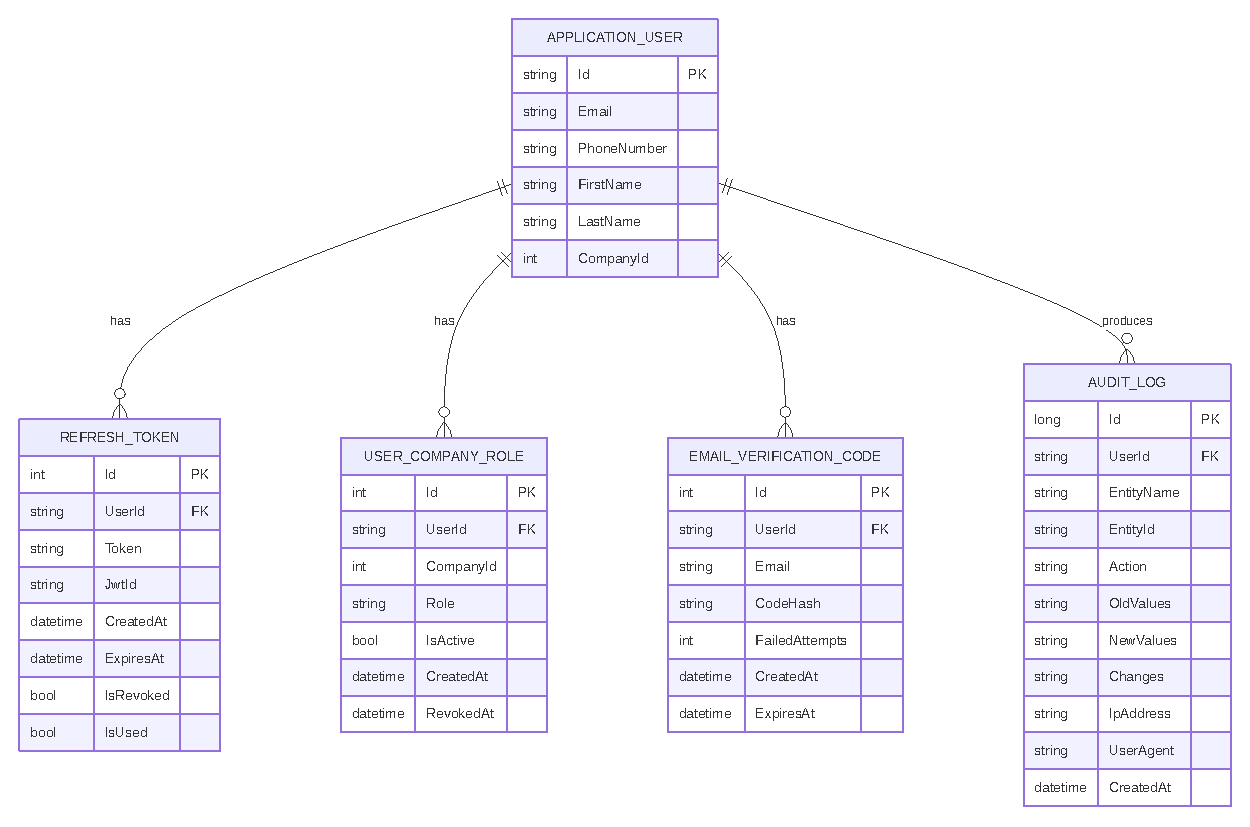
\includegraphics[width=1\textwidth]{ERD-IdentityServiceDB.pdf}
    \caption{Diagram związków encji (ERD) bazy danych mikroserwisu Identity-Service}
    \label{fig:identity_erd}
\end{figure}

\subsection{Baza danych rezerwacji (ReservationService DB)}
Na rysunku \ref{fig:reservation_erd} przedstawiono najbardziej rozbudowaną część systemu, zarządzającą logiką biznesową mikro-SaaS. Struktura wspiera model wielonajemności.

\begin{itemize}
    \item \textbf{Branches i Services:} Definiują strukturę firmy. Usługi zawierają parametry takie jak cena oraz czas trwania wraz z czasem buforowym.
    \item \textbf{Schedules i TimeSlots:} Tabele odpowiedzialne za dostępność. \textit{TimeSlot} posiada opcjonalne powiązanie z \textit{AppointmentId} – brak powiązania oznacza, że dany termin jest wolny.
    \item \textbf{Appointments:} Główna tabela rezerwacji. Implementuje mechanizm \textbf{Soft Delete}, dzięki czemu rekordy po anulowaniu nie są usuwane fizycznie, co pozwala na zachowanie spójności w tabeli \textit{BranchReviews}.
\end{itemize}

\subsection{Baza danych powiadomień (NotificationService DB)}
Baza ta została zoptymalizowana pod kątem wydajnej obsługi komunikatów i zapewnienia ich idempotentności.

\begin{itemize}
    \item \textbf{Notifications:} Przechowuje historię komunikatów \textit{In-App}, e-mail oraz SMS.
    \item \textbf{ProcessedMessages:} Kluczowa tabela dla stabilności systemu. Zawiera pole \textbf{DedupeKey}, które zapobiega ponownemu przetworzeniu tego samego zdarzenia z RabbitMQ (idempotentność konsumenta).
    \item \textbf{Templates:} Przechowuje szablony wiadomości z dynamicznymi placeholderami, które są uzupełniane danymi z pola \textit{RelatedAppointmentId}.
\end{itemize}

\begin{figure}[H]
    \centering
    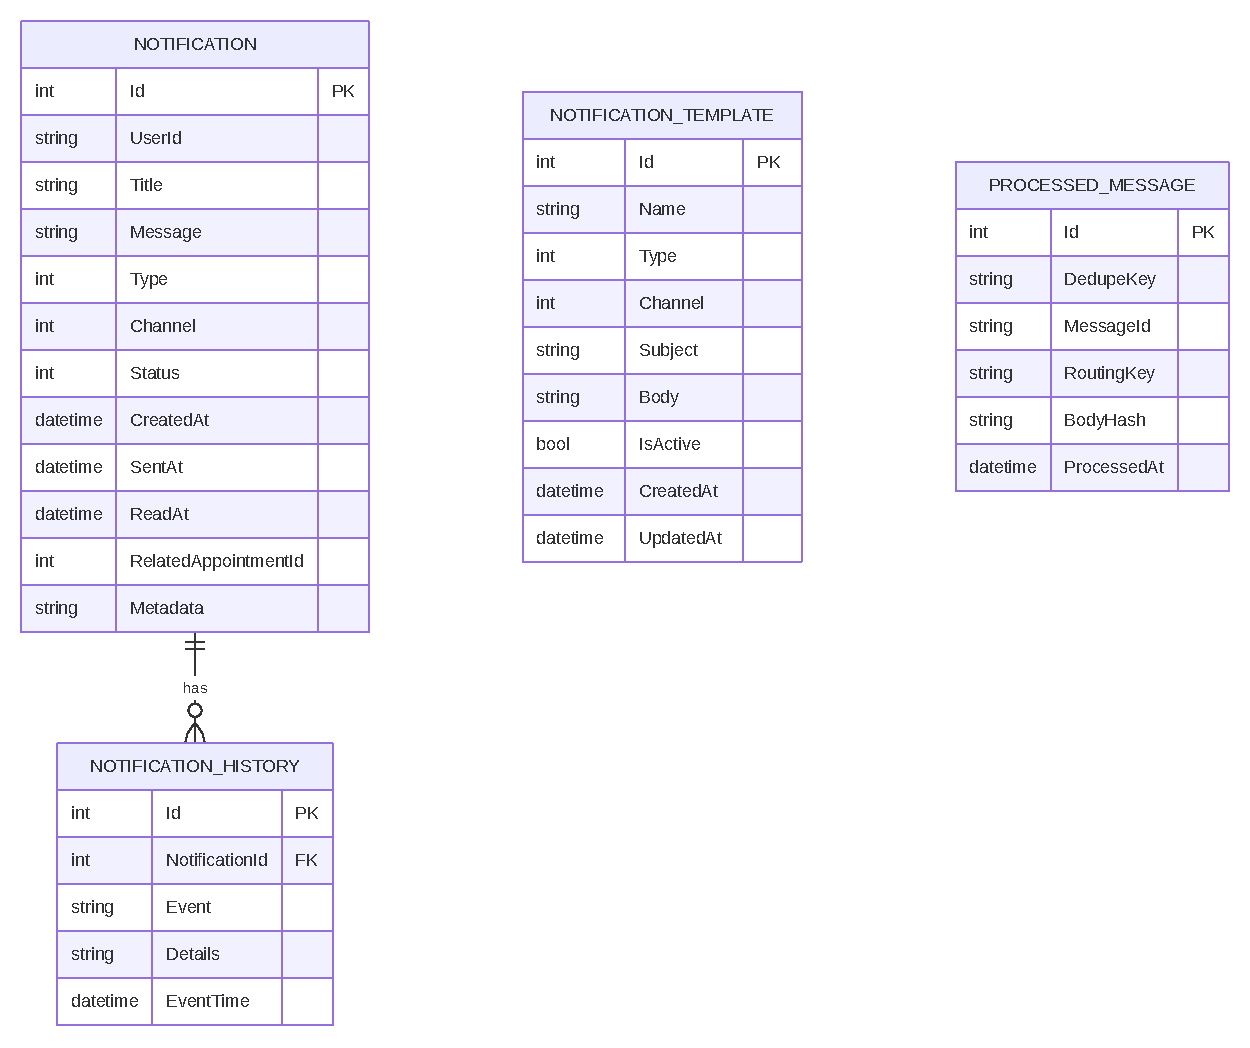
\includegraphics[width=1\textwidth]{ERD-NotificationServiceDB.pdf}
    \caption{Diagram związków encji (ERD) bazy danych mikroserwisu Notification-Service}
    \label{fig:notification_erd}
\end{figure}

\subsection{Integralność danych w architekturze rozproszonej}
Z racji fizycznej separacji baz danych, system nie wykorzystuje tradycyjnych więzów integralności (\textit{Foreign Keys}) pomiędzy serwisami. Zamiast tego zastosowano mechanizm \textbf{spójności ostatecznej} (\textit{Eventual Consistency}):
\begin{enumerate}
    \item Identyfikatory użytkowników (GUID) są przekazywane w tokenach JWT \cite{jwt_rfc} i zapisywane jako zwykłe pola typu UUID w bazie rezerwacji.
    \item Zmiany danych (np. zmiana statusu rezerwacji) są propagowane asynchronicznie przez broker komunikatów RabbitMQ \cite{rabbitmq_docs}.
    \item Mechanizm \textit{Audit Log} w każdej bazie pozwala na odtworzenie stanu systemu w przypadku niespójności.
\end{enumerate}

% Zdjecie Reservation z ograniczona wysokoscia na koncu rozdzialu
\begin{figure}[H]
    \centering
    % Ograniczenie do 20cm wysokosci przy zachowaniu proporcji
    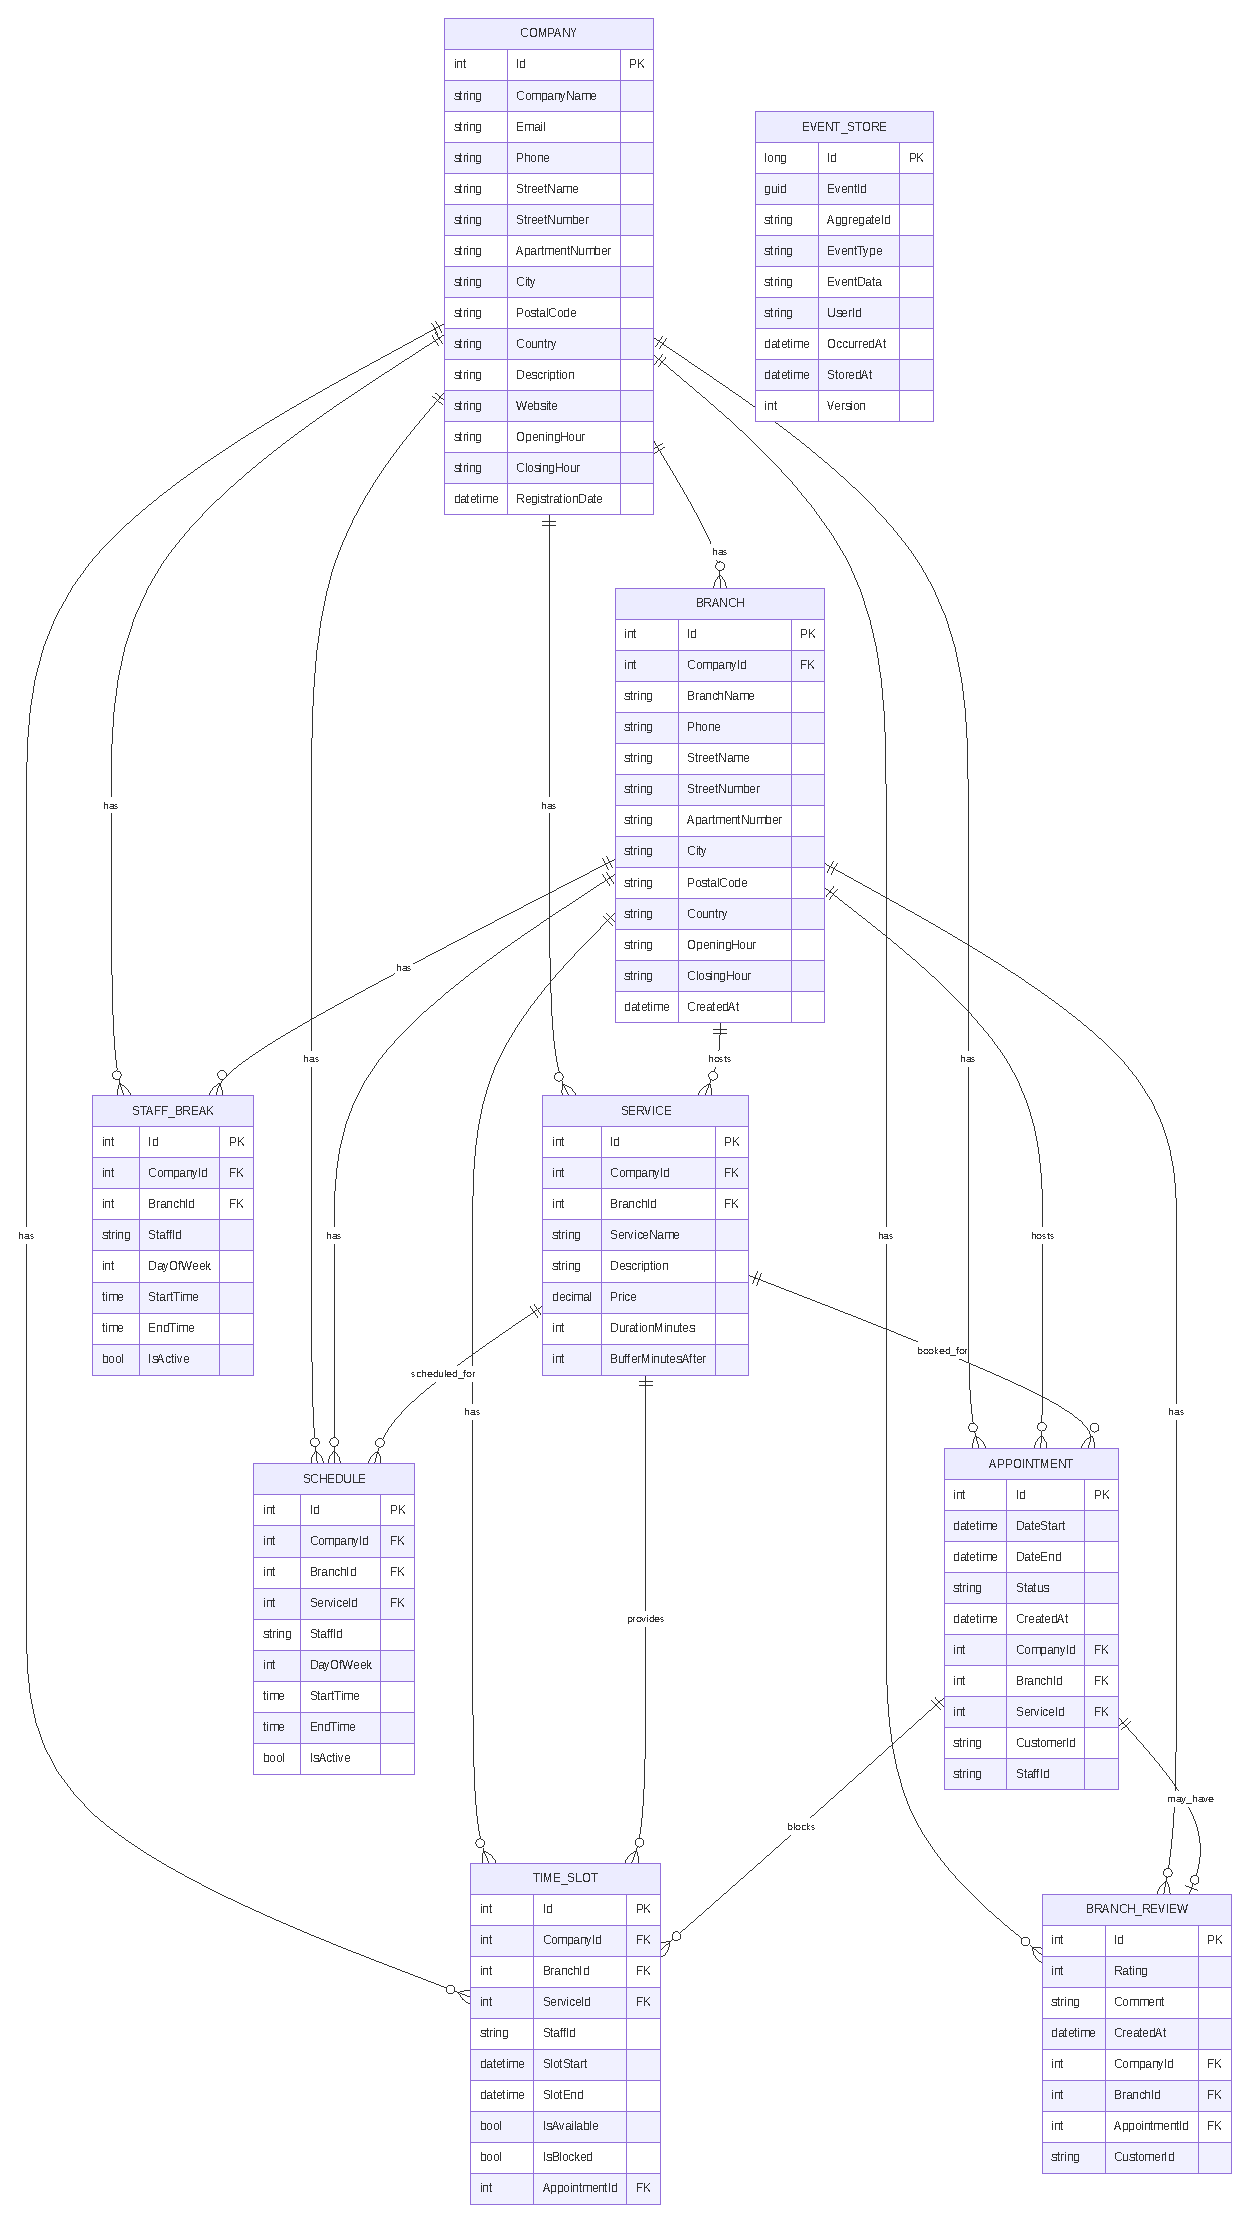
\includegraphics[height=24cm, width=1\textwidth, keepaspectratio]{ERD-ReservationServiceDB.pdf}
    \caption{Diagram związków encji (ERD) bazy danych mikroserwisu Reservation-Service}
    \label{fig:reservation_erd}
\end{figure}
\newpage
\renewcommand{\sectioncolor}{chap3}
\section{Implementacja kluczowych funkcjonalności}

\subsection{Bezpieczeństwo i zarządzanie tożsamością (JWT)}
Fundamentem bezpieczeństwa systemu jest bezstanowa autoryzacja oparta na standardzie \textit{JSON Web Token}. Proces ten został zaimplementowany w ramach \textit{Identity Service}. Mechanizm nie ogranicza się jedynie do generowania tokenów dostępu (\textit{Access Token}), ale wspiera również długotrwałe sesje poprzez tokeny odświeżania (\textit{Refresh Tokens}) przechowywane w bazie danych PostgreSQL. Pozwala to na zachowanie wysokiego poziomu bezpieczeństwa przy jednoczesnym komforcie użytkowania aplikacji.

\begin{lstlisting}[language=JavaScript, caption=Przykładowy store Zustand do zarządzania transakcjami]

\end{lstlisting}
\subsection{Zarządzanie strukturą biznesową i ofertą usług}
System umożliwia modelowanie wielooddziałowych przedsiębiorstw. Kluczowym wyzwaniem było stworzenie elastycznego katalogu usług, gdzie każda usługa może posiadać unikalne parametry, takie jak cena, czas trwania czy tzw. \textit{buffer time} (czas techniczny po wizycie). Implementacja wykorzystuje \textit{Entity Framework Core} do obsługi relacji między firmą, jej filiami a dostępnym asortymentem usług.

\begin{lstlisting}[language=JavaScript, caption=Przykładowy store Zustand do zarządzania transakcjami]

\end{lstlisting}

\subsection{Algorytm wyliczania dostępności i rezerwacji terminów}
Najbardziej złożonym elementem systemu jest moduł dynamicznego generowania dostępnych slotów czasowych. Algorytm w czasie rzeczywistym analizuje trzy źródła danych: zdefiniowane harmonogramy pracy pracowników, zarejestrowane przerwy (\textit{Staff Breaks}) oraz istniejące już rezerwacje w wybranym dniu. Wynikiem jest lista punktualnych przedziałów czasowych, które użytkownik może zarezerwować.

\begin{lstlisting}[language=JavaScript, caption=Przykładowy store Zustand do zarządzania transakcjami]

\end{lstlisting}
\subsection{Asynchroniczny obieg zdarzeń i powiadomień}
W celu odciążenia głównej logiki rezerwacji, komunikacja z użytkownikiem (np. potwierdzenie e-mail) została odseparowana za pomocą brokera \textit{RabbitMQ}. Zastosowano wzorzec \textit{Publisher-Subscriber} – po pomyślnym zapisaniu wizyty w bazie danych, wysyłane jest zdarzenie \textit{AppointmentCreated}. Jest ono konsumowane przez \textit{Notification Service}, który odpowiada za renderowanie treści na podstawie szablonów i wysyłkę SMTP.

\begin{lstlisting}[language=JavaScript, caption=Przykładowy store Zustand do zarządzania transakcjami]

\end{lstlisting}

\subsection{System opinii i ocen (\textit{Reviews})}
Po zrealizowanej usłudze, system pozwala na wystawienie oceny konkretnemu oddziałowi firmy. Moduł ten został zaimplementowany z uwzględnieniem agregacji danych – każda nowa opinia wpływa na średnią ocenę widoczną w wyszukiwarce. Zastosowanie osobnej tabeli dla recenzji pozwala na budowanie zaufania między klientami a usługodawcami.

\begin{lstlisting}[language=JavaScript, caption=Przykładowy store Zustand do zarządzania transakcjami]

\end{lstlisting}
\subsection{Dziennik audytowy i śledzenie zmian (\textit{Audit Log})}
W trosce o integralność danych, szczególnie w kontekście zarządzania pracownikami i rezerwacjami, wdrożono mechanizm audytu. Każda istotna zmiana stanu systemu (np. zmiana roli pracownika, anulowanie wizyty) jest rejestrowana w dedykowanej tabeli wraz z informacją o autorze zmiany, adresie IP oraz sygnaturze czasowej. Zapewnia to pełną transparentność działań administratorów i menedżerów.

\begin{lstlisting}[language=JavaScript, caption=Przykładowy store Zustand do zarządzania transakcjami]

\end{lstlisting}

\newpage
\renewcommand{\sectioncolor}{chap4}
\section{Warstwa prezentacji – Implementacja funkcjonalności Frontend (React)}

Warstwa kliencka systemu została zbudowana przy użyciu biblioteki \textbf{React 19}. Poniżej opisano technologiczną realizację kluczowych modułów oraz funkcjonalności interfejsu użytkownika, skupiając się na logice biznesowej i integracji z mikroserwisami.

\subsection{Moduł Użytkownika – Proces rejestracji i rezerwacji}
Interfejs klienta został zaprojektowany z myślą o prostocie obsługi. Proces rejestracji obejmuje weryfikację adresu e-mail za pomocą cyfrowego kodu OTP, co zapewnia bezpieczeństwo tożsamości. Najważniejszym elementem jest formularz rezerwacji, który dynamicznie oblicza dostępność slotów czasowych na podstawie danych z serwisu rezerwacji.

\begin{lstlisting}[language=JavaScript, caption={Walidacja danych kontaktowych oraz filtrowanie slotów (BookingPage.js)}]
const validateContact = (next) => {
  const email = String(next.customerEmail || "").trim();
  const phone = sanitizePhoneNumberInput(next.customerPhone);

  const emailOk = !email || /^[^\s@]+@[^\s@]+\.[^\s@]+$/.test(email);
  const phoneOk = !phone || /^\+\d{8,15}$/.test(phone);

  return {
    customerEmail: emailOk ? "" : "booking.invalidEmail",
    customerPhone: phoneOk ? "" : "booking.invalidPhone"
  };
};

const filteredAvailableSlots = useMemo(() => {
  if (!form.date || !form.staffId) return [];
  return availableSlots.filter((s) => 
    String(s.staffId || "") === String(form.staffId)
  );
}, [availableSlots, form.date, form.staffId]);
\end{lstlisting}

\subsection{Zarządzanie profilem i Dashboard klienta}
Użytkownik po zalogowaniu ma dostęp do pulpitu (\textit{Dashboard}), który agreguje informacje o nadchodzących wizytach. System umożliwia również zarządzanie danymi profilowymi, wykorzystując zaawansowane funkcje normalizacji danych wejściowych, co gwarantuje spójność bazy danych.

\begin{lstlisting}[language=JavaScript, caption={Normalizacja kodu pocztowego i formatowanie numeru telefonu (AccountPage.js)}]
const normalizePostalCodeInput = (value) => {
  const digits = String(value || '').replace(/\D/g, '').slice(0, 5);
  if (digits.length <= 2) return digits;
  return `${digits.slice(0, 2)}-${digits.slice(2)}`;
};

const formatPhoneDisplay = (value) => {
  const raw = String(value || '').trim();
  const digits = raw.replace(/\D/g, '').slice(0, 12);
  if (!digits) return raw.startsWith('+') ? '+' : '';
  
  const country = digits.slice(0, 3);
  const rest = digits.slice(3);
  const groups = rest.match(/.{1,3}/g) || [];
  return `+${country} ${groups.join('-')}`;
};
\end{lstlisting}

\subsection{Moduł Firmowy – Zarządzanie uprawnieniami i kadrą}
Panel administracyjny firmy dynamicznie dostosowuje zakres dostępnych funkcjonalności na podstawie roli użytkownika (RBAC – \textit{Role-Based Access Control}). Logika frontendu rozróżnia uprawnienia właściciela (\textit{Owner}), managera oraz pracownika.

\begin{lstlisting}[language=JavaScript, caption={Logika weryfikacji uprawnień wewnątrz organizacji (CompanyPanel.js)}]
const companyRole = tokenManager.getUser()?.companyRole;
const userRoles = tokenManager.getUser()?.roles || [];
const isAdmin = userRoles.includes("Admin");
const isOwner = companyRole === "Owner";
const isManager = companyRole === "Manager";

// Definicja dostępu do akcji krytycznych
const canManageEmployees = isAdmin || isOwner || isManager;
const canEditCompany = isAdmin || isOwner;

const handleUpdateUserRole = async (userId, newRole) => {
  try {
    await companyUsersAPI.updateUserRole(userId, newRole);
    await loadEmployees();
  } catch (err) {
    console.error("Failed to update role", err);
  }
};
\end{lstlisting}

\subsection{Zarządzanie harmonogramami i przerwami pracowników}
Ważną funkcjonalnością jest wizualizacja czasu pracy. Użytkownik może definiować dni i godziny pracy oraz konfigurować przerwy (\textit{Staff Breaks}). Do obsługi wielodniowych harmonogramów wykorzystano komponent zarządzający kolekcją dni.

\begin{lstlisting}[language=JavaScript, caption={Obsługa komponentu wyboru dni tygodnia (CompanyPanel.js)}]
const toggleDay = (day) => {
  const d = Number(day);
  const current = normalizeDays(normalizedValue);
  const next = current.includes(d) 
    ? current.filter((x) => x !== d) 
    : [...current, d];
  onChange(normalizeDays(next));
};

const handleCreateStaffBreak = async (e) => {
  e.preventDefault();
  const daysToCreate = normalizeDays(staffBreakFilters.dayOfWeek);
  await Promise.all(
    daysToCreate.map((d) => staffBreaksAPI.create({ ...payload, dayOfWeek: d }))
  );
};
\end{lstlisting}

\subsection{Moduł Administracyjny i szablony powiadomień}
Administratorzy systemowi zarządzają szablonami wiadomości, które wspierają dynamiczne wstrzykiwanie zmiennych. Pozwala to na personalizację powiadomień e-mail i SMS wysyłanych przez mikroserwis powiadomień.

\begin{lstlisting}[language=JavaScript, caption={Mechanizm wstawiania tokenów do edytora szablonów (AdminPanel.js)}]
const insertTemplateToken = (token) => {
  const field = activeTemplateField === "subject" ? "subject" : "body";
  const el = field === "subject" ? subjectRef.current : bodyRef.current;
  const currentValue = String(editingTemplate?.[field] ?? "");

  if (el && typeof el.selectionStart === "number") {
    const start = el.selectionStart;
    const end = el.selectionEnd;
    const next = `${currentValue.slice(0, start)}${token}${currentValue.slice(end)}`;
    handleTemplateFormChange(field, next);
  }
};
\end{lstlisting}

\subsection{Integracja z geokodowaniem i mapami}
W widoku szczegółów usługi zaimplementowano interaktywną mapę \textbf{OpenStreetMap}. System przelicza adres tekstowy na współrzędne geograficzne i wyświetla lokalizację salonu w komponencie \textit{iframe}, co znacząco poprawia użyteczność aplikacji.

\begin{lstlisting}[language=JavaScript, caption={Geokodowanie adresu i generowanie widoku mapy (ServiceDetailsPage.js)}]
useEffect(() => {
  const geocode = async () => {
    try {
      const res = await geocodeAPI.geocode(osmQuery);
      if (res.data?.found) {
        setMapCoords({ lat: res.data.lat, lon: res.data.lon });
      }
    } catch (err) {
      setMapCoords(null);
    }
  };
  if (osmQuery) geocode();
}, [osmQuery]);
\end{lstlisting}
\newpage
\renewcommand{\sectioncolor}{chap5}
\section{Konteneryzacja i środowisko uruchomieniowe}

W celu zapewnienia powtarzalności środowiska oraz uproszczenia procesu wdrażania, system został w pełni skonteneryzowany przy użyciu technologii \textbf{Docker} \cite{docker_docs}. Pozwala to na izolację poszczególnych mikroserwisów wraz z ich zależnościami w lekkich kontenerach, co eliminuje problem różnic między środowiskami programistycznymi a produkcyjnymi. Obrazy wynikowe są przechowywane i zarządzane w ramach rejestru \textit{GitHub Container Registry} \cite{ghcr_guide}.

\subsection{Konfiguracja wielokontenerowa (Docker Compose)}
Do zarządzania całym ekosystemem usług wykorzystano narzędzie \textbf{Docker Compose}. Pozwala ono na zdefiniowanie wszystkich komponentów systemu (mikroserwisy, bazy danych, brokerzy komunikatów) w jednym pliku konfiguracyjnym \texttt{docker-compose.yml} oraz ich jednoczesne uruchomienie przy pomocy jednej komendy.

\begin{lstlisting}[language=bash, caption={Uruchomienie całego stosu technologicznego systemu}]
# Budowa obrazów i uruchomienie kontenerów w tle
docker-compose up --build -d
\end{lstlisting}

\subsection{Charakterystyka zdefiniowanych usług}
Zgodnie z architekturą systemu, w pliku konfiguracyjnym zdefiniowano następujące grupy usług:

\begin{itemize}
    \item \textbf{Infrastruktura danych (PostgreSQL):} Wykorzystano obraz \textit{postgres:15-alpine} \cite{postgresql_docs}. Kontener został skonfigurowany tak, aby przy starcie automatycznie tworzył trzy odrębne bazy danych (\texttt{identitydb}, \texttt{reservationdb}, \texttt{notificationdb}) za pomocą skryptu inicjalizacyjnego. Trwałość danych zapewniono poprzez wolumeny (\textit{Volumes}).
    \item \textbf{Broker komunikatów (RabbitMQ):} Zastosowano obraz z panelem zarządzania (\textit{management-alpine}) \cite{rabbitmq_docs}, co pozwala na monitorowanie kolejek zdarzeń w czasie rzeczywistym na porcie 15672.
    \item \textbf{Warstwa mikroserwisów (.NET):} Serwisy \textit{Identity}, \textit{Reservation} oraz \textit{Notification} są budowane z lokalnych plików \texttt{Dockerfile} w oparciu o SDK .NET 8 \cite{dotnet_microsoft}. 
    \item \textbf{API Gateway (Ocelot):} Wykorzystano bibliotekę Ocelot \cite{ocelot_docs}, która pełni rolę centralnego punktu wejścia, mapując zewnętrzny port 5000 na wewnętrzną infrastrukturę kontenerów.
    \item \textbf{Narzędzia pomocnicze (MailHog):} Kontener służący do przechwytywania i testowania wiadomości e-mail w środowisku deweloperskim, co pozwala na bezpieczną weryfikację systemu powiadomień bez wysyłki realnych wiadomości.
\end{itemize}

[Image of Docker Compose architecture for microservices showing PostgreSQL, RabbitMQ, and .NET containers connected via a bridge network]

\subsection{Zarządzanie zależnościami i Healthchecks}
W konfiguracji zastosowano mechanizm \textbf{Healthcheck}, który monitoruje stan gotowości usług krytycznych. Mikroserwisy posiadają instrukcję \texttt{depends\_on} z warunkiem \texttt{service\_healthy}, co gwarantuje, że aplikacja .NET spróbuje nawiązać połączenie z bazą dopiero wtedy, gdy silnik bazy danych przejdzie pomyślnie test gotowości.

\begin{lstlisting}[language=yaml, caption={Fragment konfiguracji Docker Compose obsługujący zależności}]
reservation_api:
  build:
    context: ./ReservationService
  depends_on:
    postgres_db:
      condition: service_healthy
    rabbitmq:
      condition: service_healthy
\end{lstlisting}

\subsection{Izolacja sieciowa}
Wszystkie kontenery działają w ramach dedykowanej sieci wirtualnej typu \textit{bridge}. Pozwala to na komunikację między serwisami przy użyciu nazw ich usług (np. \texttt{Host=postgres\_db}) zamiast zmiennych adresów IP. Takie rozwiązanie zapewnia bezpieczną izolację — bazy danych nie są wystawione na świat zewnętrzny, a dostęp do nich mają wyłącznie autoryzowane mikroserwisy wewnątrz sieci Docker.

\subsection{Automatyzacja zarządzania systemem (Skrypty Manage)}
W celu maksymalnego uproszczenia pracy z systemem, przygotowano dedykowane skrypty zarządcze: \texttt{manage.bat} (dla systemu Windows) oraz \texttt{manage.sh} (dla systemów Unix). Stanowią one warstwę abstrakcji nad surowymi komendami silnika Docker oraz narzędzia Vite \cite{vite_guide}.

\begin{lstlisting}[language=bash, caption={Uruchomienie kompletnego środowiska za pomocą skryptu zarządczego}]
# Uruchomienie backendu w kontenerach oraz frontendu React
manage.bat all
\end{lstlisting}

Wykorzystanie powyższego skryptu wykonuje sekwencyjnie następujące zadania:
\begin{itemize}
    \item \textbf{Weryfikacja środowiska:} Sprawdzenie dostępności niezbędnych narzędzi (Docker, Node.js).
    \item \textbf{Orkiestracja kontenerów:} Wywołanie \texttt{docker-compose} w celu zbudowania i uruchomienia infrastruktury.
    \item \textbf{Uruchomienie warstwy prezentacji:} Automatyczny start serwera deweloperskiego Vite \cite{vite_guide} dla aplikacji frontendowej.
\end{itemize}

Dzięki tej automatyzacji proces wdrożenia i testowania (w tym skanowanie podatności obrazów narzędziem Trivy \cite{trivy_security}) został zintegrowany z procesem ciągłej integracji w GitHub Actions \cite{github_actions_docs}.
\newpage
\renewcommand{\sectioncolor}{chap6}
\section{Testowanie i proces CI/CD}

Kluczowym elementem wytwarzania nowoczesnego oprogramowania jest zapewnienie jego jakości poprzez automatyzację procesów weryfikacyjnych. W niniejszym systemie zaimplementowano wielopoziomowe podejście do testowania oraz potok ciągłej integracji (ang. \textit{Continuous Integration}).

\subsection{Testy automatyczne}
System został objęty testami automatycznymi zarówno w warstwie serwerowej, jak i klienckiej, co pozwala na szybkie wykrywanie błędów regresji.

\subsubsection{Testy warstwy backendowej (xUnit)}
Dla mikroserwisów Identity, Reservation oraz Notification przygotowano dedykowane projekty testowe wykorzystujące framework \textbf{xUnit} \cite{xunit_doc}. Testy te skupiają się na weryfikacji logiki biznesowej, poprawności mapowania obiektów oraz działaniu punktów końcowych API.

\begin{itemize}
    \item \textbf{Walidacja domeny:} Sprawdzanie reguł biznesowych, np. zakazu rezerwacji terminów w przeszłości.
    \item \textbf{Testy integracyjne:} Weryfikacja poprawnej komunikacji z bazą danych PostgreSQL przy użyciu biblioteki Entity Framework Core \cite{ef_core_testing}.
\end{itemize}

\subsubsection{Testy warstwy frontendowej (Vitest)}
W części klienckiej zastosowano nowoczesny framework testowy \textbf{Vitest} \cite{vitest_guide}. Testy obejmują kluczowe komponenty interfejsu użytkownika oraz mechanizmy nawigacji.

\begin{itemize}
    \item \textbf{Weryfikacja komponentów:} Testowanie renderowania elementów interfejsu takich jak ikony i przyciski nawigacyjne.
    \item \textbf{Logika autoryzacji:} Testowanie ochrony ścieżek (\textit{ProtectedRoute}), zapewniające, że nieautoryzowani użytkownicy nie mają dostępu do paneli administracyjnych.
\end{itemize}

\subsection{Potok CI/CD w środowisku GitHub Actions}
Proces integracji i wdrażania został w pełni zautomatyzowany przy użyciu usługi \textbf{GitHub Actions} \cite{github_actions_docs}. Skonfigurowany potok (\textit{pipeline}) uruchamia się automatycznie przy każdym zdarzeniu \textit{push} lub \textit{pull request}.



Proces CI obejmuje następujące etapy:
\begin{enumerate}
    \item \textbf{Przywracanie i budowa (Restore \& Build):} Automatyczne pobieranie zależności bibliotecznych oraz kompilacja kodu źródłowego mikroserwisów i aplikacji frontendowej.
    \item \textbf{Uruchomienie testów:} Wykonanie wszystkich testów jednostkowych i integracyjnych. Niepowodzenie któregokolwiek z nich skutkuje przerwaniem procesu wdrażania.
    \item \textbf{Skanowanie bezpieczeństwa (Security Scan):} Wykorzystanie narzędzia \textbf{Trivy} \cite{trivy_security} do analizy obrazów i kodu pod kątem znanych podatności (CVE).
    \item \textbf{Budowa obrazów (Build Images):} Po pomyślnym przejściu testów, system buduje obrazy kontenerowe i publikuje je w rejestrze \textbf{GHCR} \cite{ghcr_guide}.
\end{enumerate}

\subsection{Weryfikacja integracyjna (Smoke Tests)}
Poza testami jednostkowymi, wdrożono skrypty typu \textbf{Smoke Tests}. Ich zadaniem jest uruchomienie całego stosu technologicznego i sprawdzenie podstawowej drożności systemu, w tym:
\begin{itemize}
    \item Poprawności działania routingu w \textbf{API Gateway}.
    \item Sprawdzenia dostępności (\textit{health check}) wszystkich punktów końcowych API mikroserwisów.
    \item Symulacji kluczowych kroków procesu rezerwacji i autentykacji.
\end{itemize}
\newpage
\renewcommand{\sectioncolor}{chap6}
\section{Podsumowanie i perspektywy rozwoju}

Niniejsza praca pozwoliła na zaprojektowanie i zaimplementowanie skalowalnego systemu rezerwacji usług w modelu Mikro-SaaS. Wykorzystanie architektury mikroserwisowej opartej na platformie .NET 8 \cite{dotnet_microsoft} oraz bibliotece React 19 \cite{react_meta} umożliwiło stworzenie rozwiązania charakteryzującego się wysoką wydajnością oraz czytelnym podziałem odpowiedzialności między poszczególnymi modułami.

\subsection{Wnioski z realizacji projektu}
Proces wytwórczy oraz przeprowadzone testy automatyczne \cite{vitest_guide} pozwoliły na sformułowanie następujących wniosków inżynierskich:

\begin{itemize}
    \item \textbf{Efektywność komunikacji asynchronicznej:} Zastosowanie brokera komunikatów RabbitMQ \cite{rabbitmq_docs} pozwoliło na całkowite odseparowanie serwisu rezerwacji od modułu powiadomień. Dzięki temu proces rezerwacji terminu nie jest blokowany przez czasochłonne operacje wysyłki wiadomości e-mail.
    \item \textbf{Izolacja danych:} Model \textit{Database-per-Service} z wykorzystaniem bazy PostgreSQL \cite{postgresql_docs} zagwarantował, że błędy w obrębie jednego schematu danych (np. logów powiadomień) nie wpływają na stabilność krytycznych tabel rezerwacji.
    \item \textbf{Wydajność interfejsu:} Wykorzystanie narzędzia Vite \cite{vite_guide} oraz mechanizmów normalizacji danych wejściowych (np. telefonów i kodów pocztowych) znacząco poprawiło komfort pracy użytkownika (\textit{User Experience}) oraz jakość danych trafiających do systemu.
    \item \textbf{Bezpieczeństwo:} Implementacja mechanizmu \textit{Refresh Tokens} oraz centralna walidacja JWT na poziomie API Gateway \cite{ocelot_docs} zapewniły standard bezpieczeństwa zgodny z zaleceniami RFC 7519 \cite{jwt_rfc}.
\end{itemize}

\subsection{Kierunki dalszego rozwoju systemu}
Choć system w obecnej fazie jest w pełni funkcjonalny, architektura pozwala na jego dalszą rozbudowę w następujących obszarach:

\begin{itemize}
    \item \textbf{Integracja z kalendarzami zewnętrznymi:} Implementacja dwukierunkowej synchronizacji z Google Calendar oraz Outlook za pomocą dedykowanych API.
    \item \textbf{System płatności online:} Integracja z platformą Stripe \cite{axios_docs} w celu umożliwienia pobierania przedpłat za rezerwacje oraz zarządzania subskrypcjami firm korzystających z modelu SaaS.
    \item \textbf{Aplikacja mobilna:} Stworzenie natywnego interfejsu dla pracowników w technologii React Native, co ułatwiłoby zarządzanie harmonogramem w terenie.
    \item \textbf{Rozbudowa modułu powiadomień:} Dodanie obsługi wiadomości SMS oraz powiadomień typu \textit{Push} z wykorzystaniem technologii SignalR \cite{signalr_microsoft}.
\end{itemize}

\subsection{Podsumowanie końcowe}
Projekt udowodnił, że zastosowanie wzorców takich jak CQRS, API Gateway oraz komunikacja sterowana zdarzeniami pozwala na budowę systemów gotowych do obsługi dużego ruchu i wielu niezależnych organizacji jednocześnie. Praca nad systemem pozwoliła na zdobycie praktycznego doświadczenia w zakresie orkiestracji kontenerów Docker \cite{docker_docs} oraz automatyzacji procesów CI/CD \cite{github_actions_docs}, co stanowi solidną podstawę dla nowoczesnej inżynierii oprogramowania.



% === BIBLIOGRAFIA ===
\newpage
\renewcommand{\sectioncolor}{black}

% Ustawienie stylu bibliografii na IEEE Transaction
\bibliographystyle{IEEEtran}

% Wskazanie pliku bazy bibliograficznej
\bibliography{bibliografia.bib}


\end{document}